\subsection{Artifical Weather Effects}
Inspired by \cite{weather-effects-tutorial}, we implemented the following
natural-looking weather effects with OpenCV to verify the generalization of our
method, and improve training:
\begin{itemize}
    \item \emph{light-rain:} A little blur to the image and random generated lines
    \item \emph{normal-rain:} Same as light-rain, but more lines
    \item \emph{snow:} Change the color of some part of picture to white to simulate snow.
    \item \emph{sun:} Increase brightness for simulating a sunny day
\end{itemize}

We show these effects in action in Figure~\ref{fig:weather-effects}.

\begin{figure}
    \begin{subfigure}[b]{\textwidth}
        \centering
        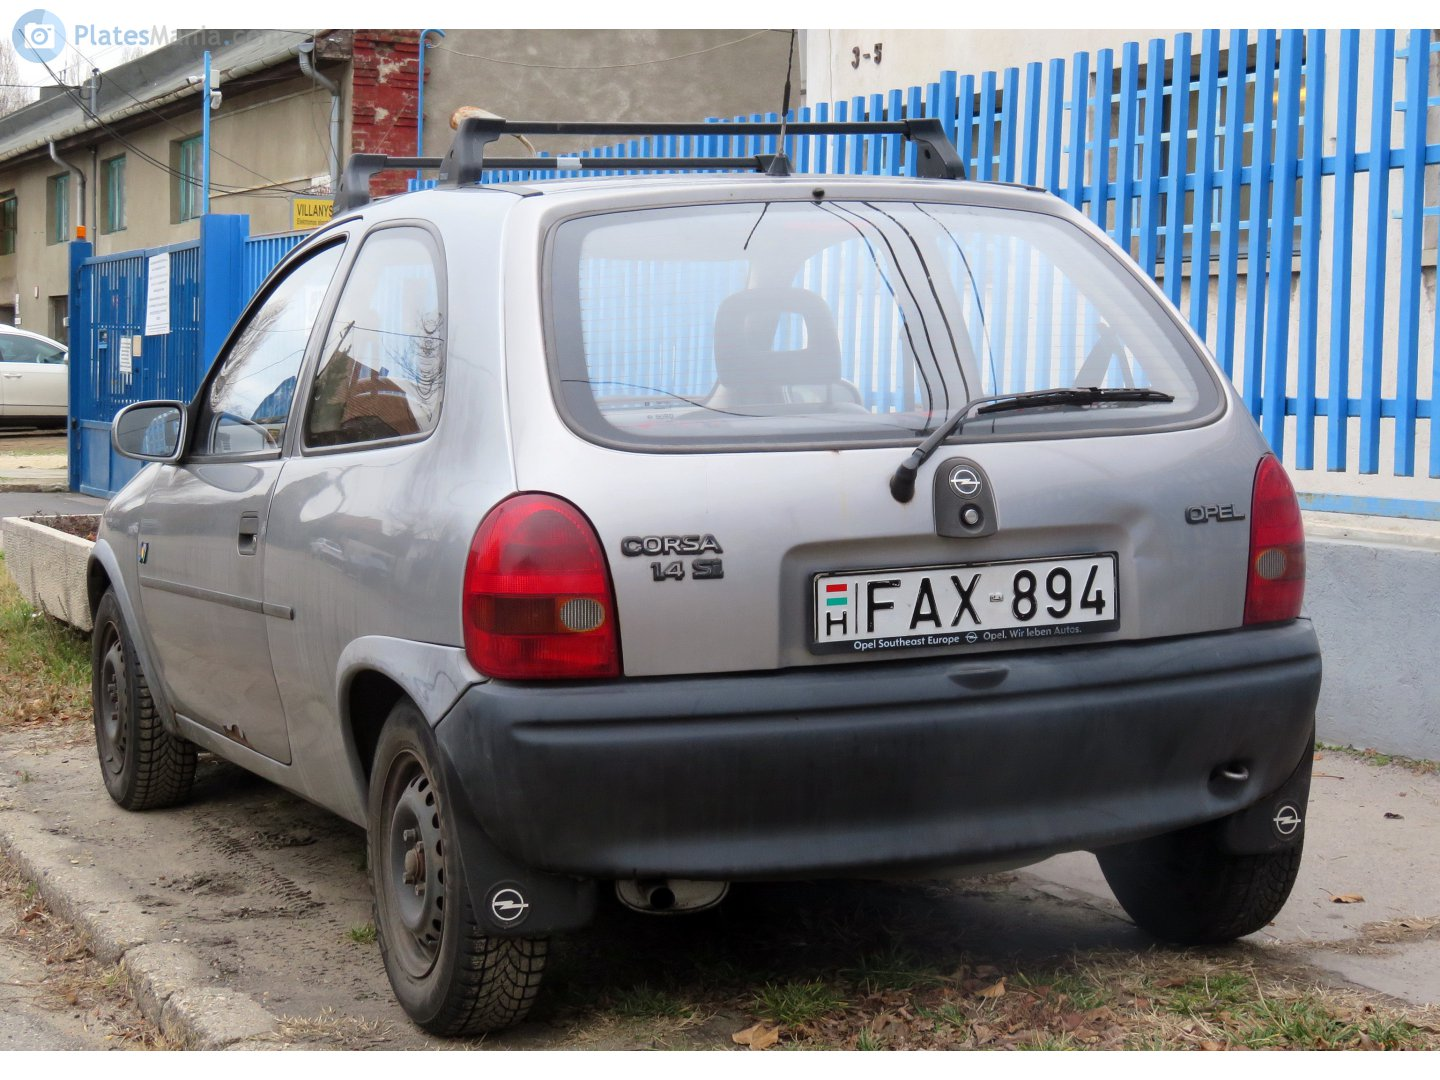
\includegraphics[width=0.4\textwidth]{figures/original.jpg}
        \begin{subfigure}[b]{0.4\textwidth}
            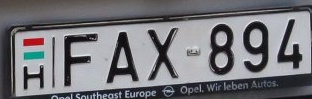
\includegraphics[width=\textwidth]{figures/weather-results/cutouts/original_0.jpg}
            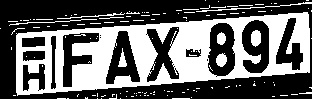
\includegraphics[width=\textwidth]{figures/weather-results/cleared/original_0.jpg}
        \end{subfigure}
        \caption{Original Image}
        \label{fig:weather-original}
    \end{subfigure}
    \begin{subfigure}[t]{\textwidth}
        \centering
        \begin{subfigure}[t]{.4\textwidth}
            \centering
            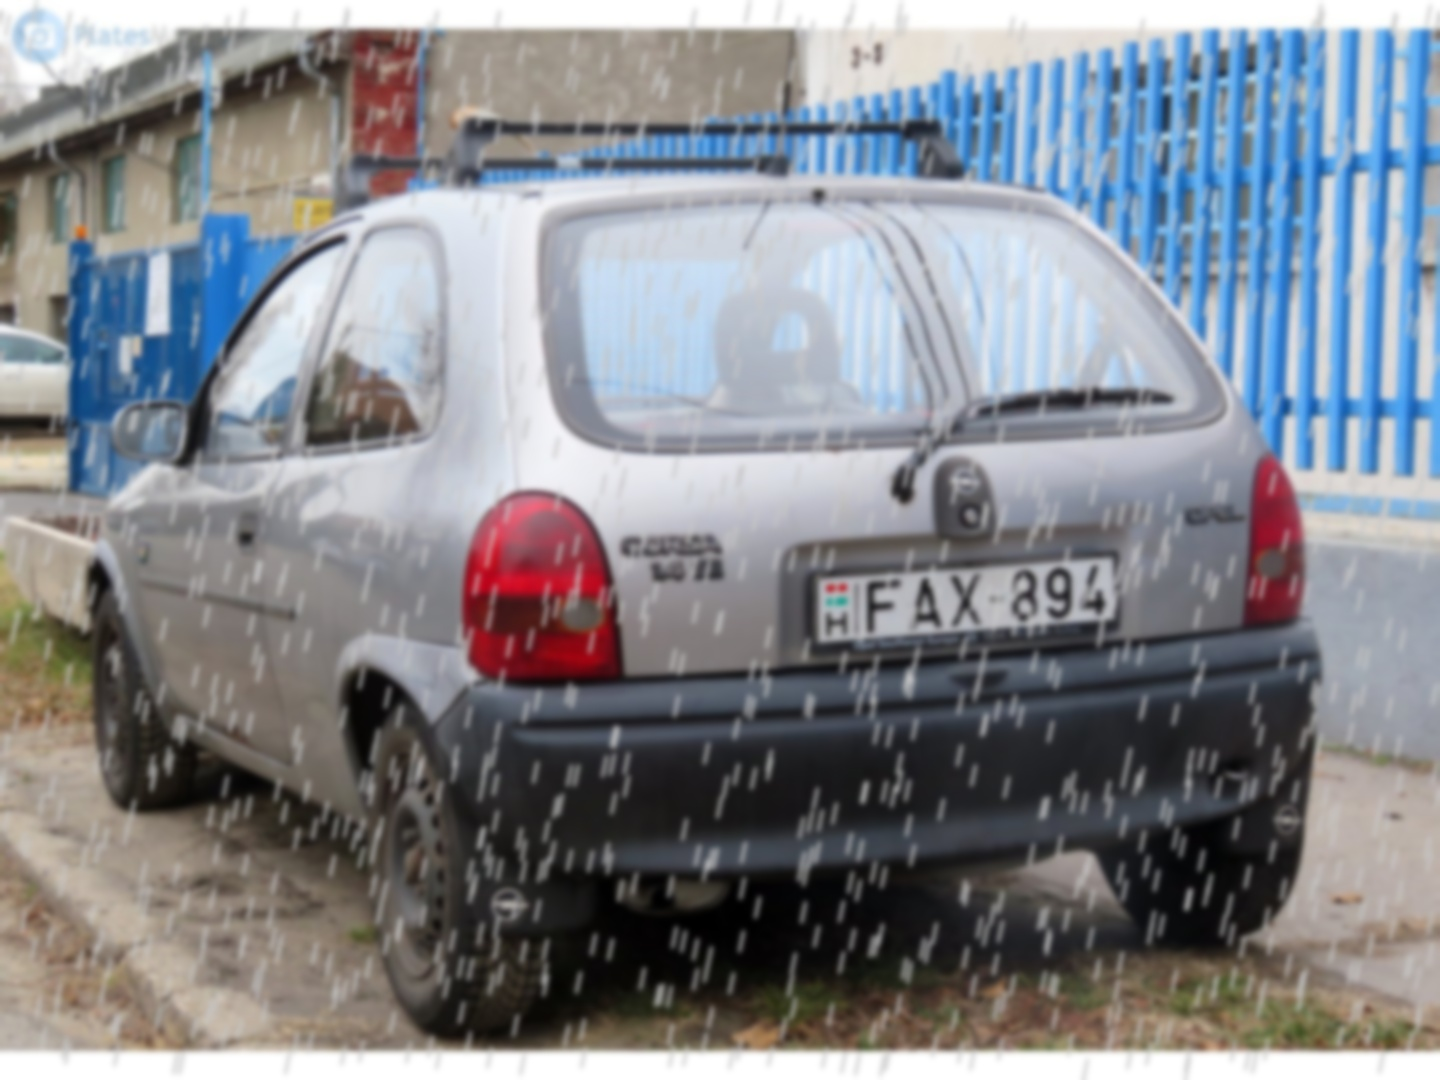
\includegraphics[width=\textwidth]{figures/lightrain.jpg}
            
\includegraphics[width=0.45\textwidth]{figures/weather-results/cutouts/lightrain_0.jpg}
            
\includegraphics[width=0.45\textwidth]{figures/weather-results/cleared/lightrain_0.jpg}
            \caption{Light rain. Although the object detection correctly
                recognizes the license plate present in the scene, our OCR fails
                to correctly recognize the letters. This can be due to our
                preprocessing step introducing unwanted artifacts.}
        \end{subfigure}
        \begin{subfigure}[t]{.4\textwidth}
            \centering
            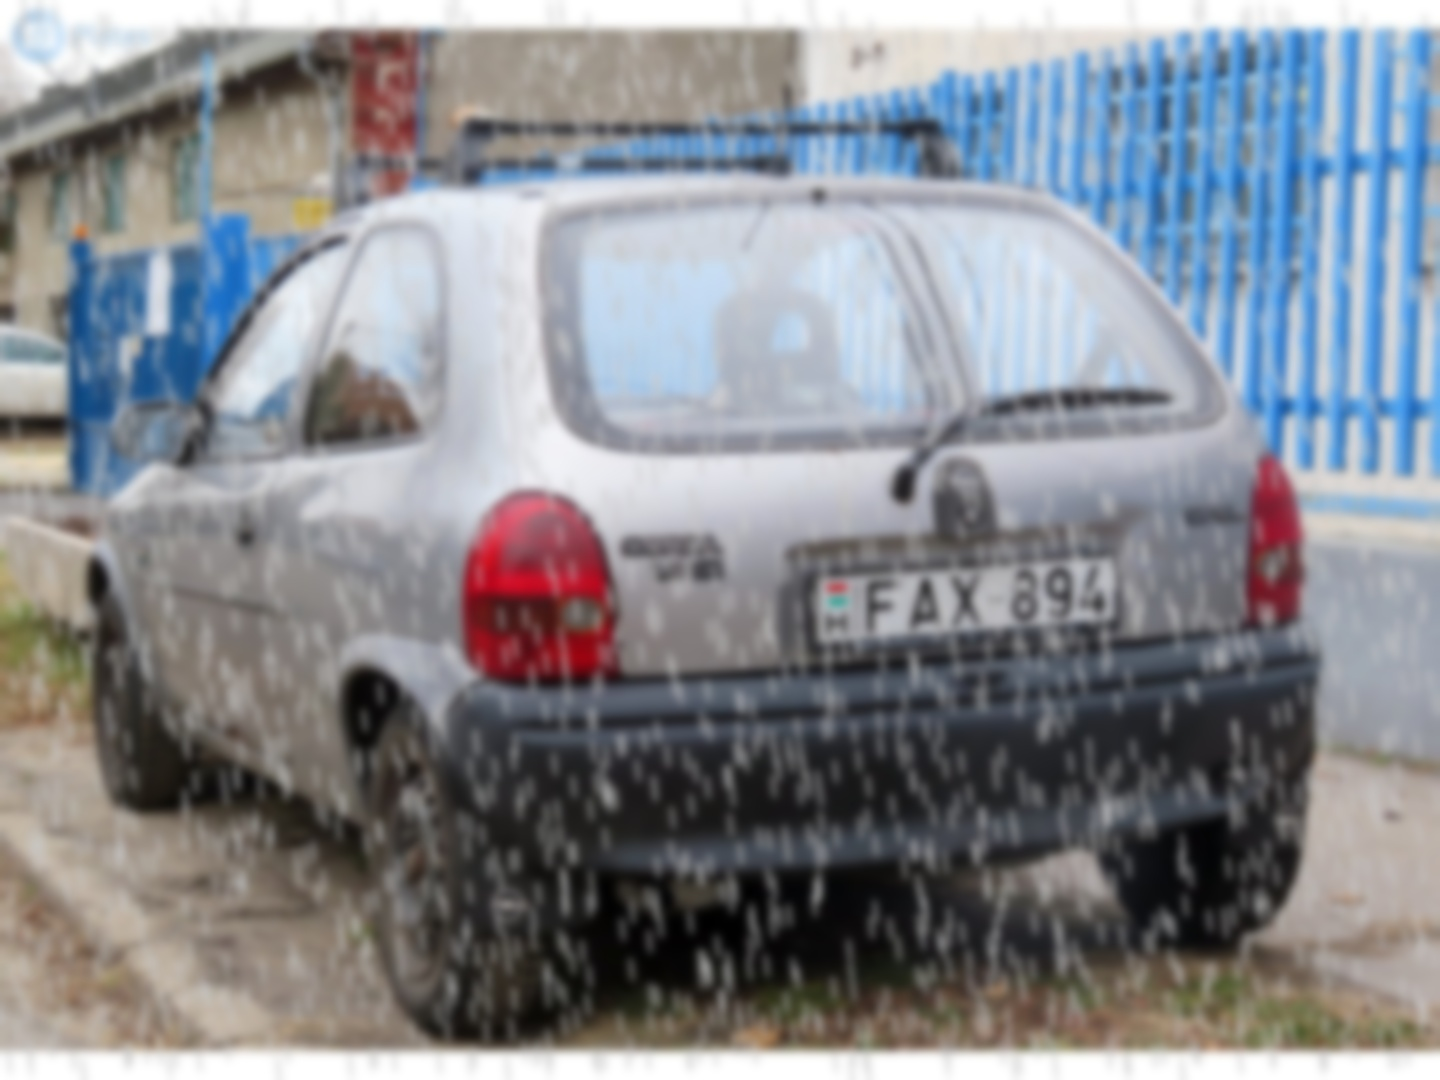
\includegraphics[width=\textwidth]{figures/rain.jpg}
            \caption{Heavy rain. Even the object detection fails to pick up on
            the license plate present in the scene.}
        \end{subfigure}
        \label{fig:weather-rains}
    \end{subfigure}
    \begin{subfigure}[b]{\textwidth}
        \centering
        \begin{subfigure}[b]{.4\textwidth}
            \centering
            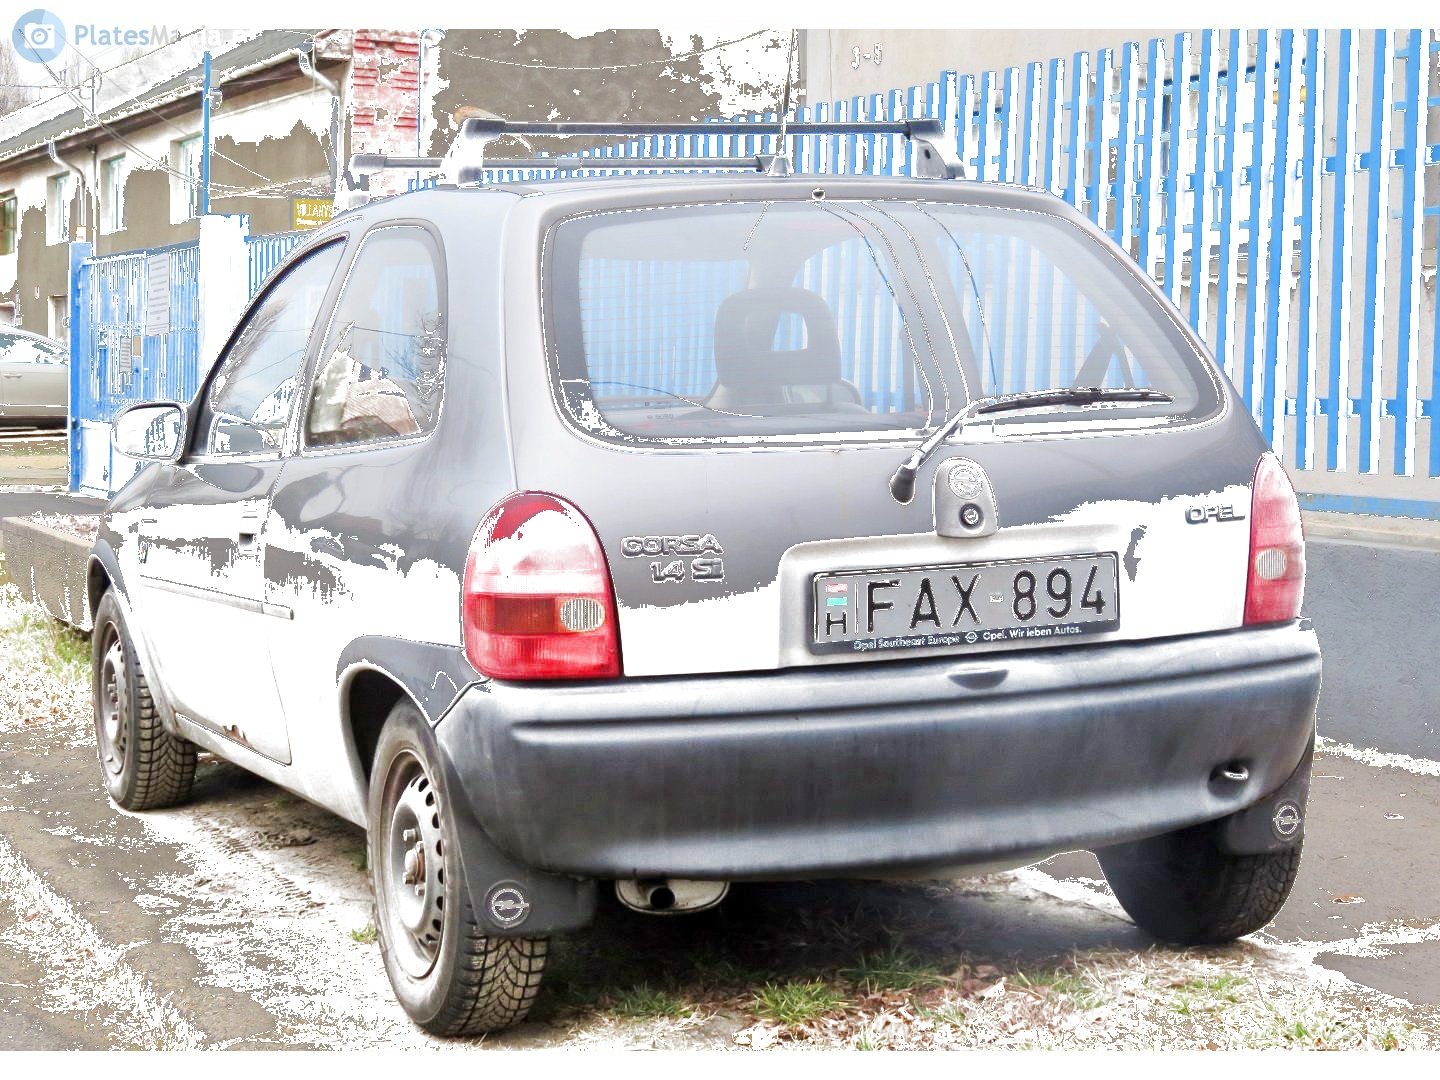
\includegraphics[width=\textwidth]{figures/snow.jpg}
            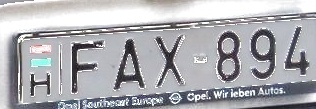
\includegraphics[width=0.45\textwidth]{figures/weather-results/cutouts/snow_0.jpg}
            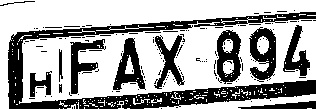
\includegraphics[width=0.45\textwidth]{figures/weather-results/cleared/snow_0.jpg}
        \end{subfigure}
        \begin{subfigure}[b]{.4\textwidth}
            \centering
            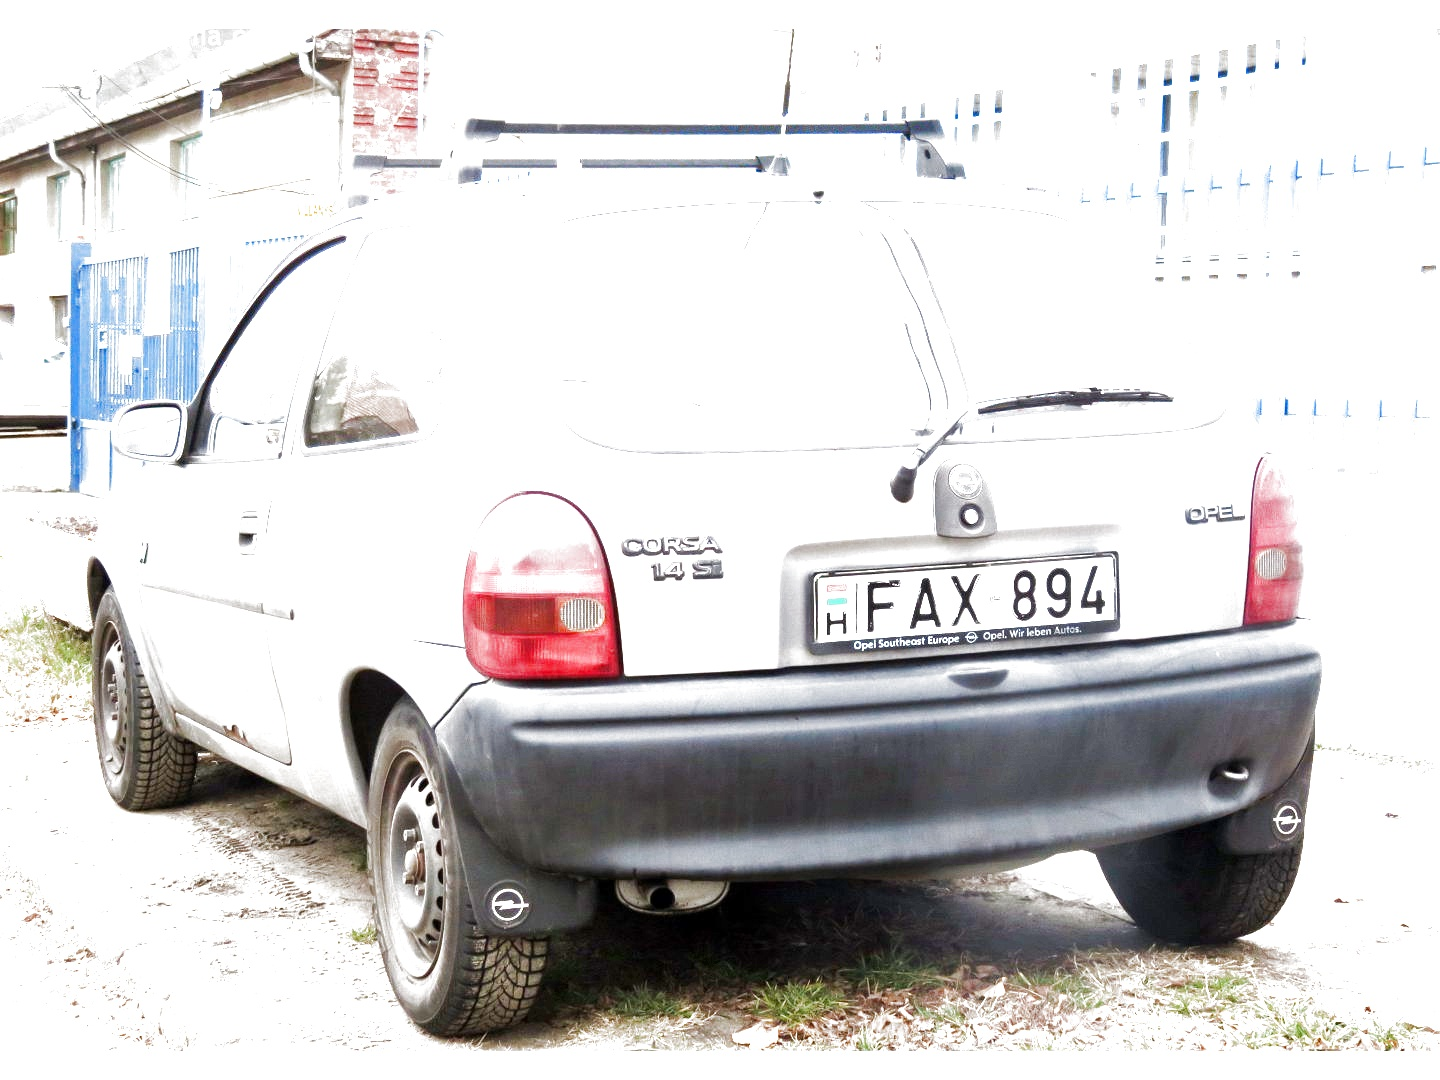
\includegraphics[width=\textwidth]{figures/sunny.jpg}
            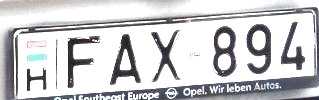
\includegraphics[width=0.45\textwidth]{figures/weather-results/cutouts/sunny_0.jpg}
            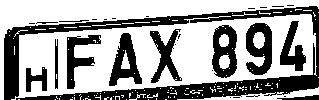
\includegraphics[width=0.45\textwidth]{figures/weather-results/cleared/sunny_0.jpg}
        \end{subfigure}
        \caption{Snow and Sun filter. The object detection stage of our pipeline
            performs well in both cases, although the OCR fails to correctly
            recognize the letters under sunny conditions.}
        \label{fig:weather-snow-sun}
    \end{subfigure}
    \caption{Different types of natural-looking weather effects, and
    corresponding immediate results: original cut out from the object detection
    step, and the preprocessing step, that serves as the input to the OCR step.}
    \label{fig:weather-effects}
\end{figure}

